\documentclass[border=0pt]{standalone}
% Match the Computer Modern text and mathematics of main.tex and its circuits.
\usepackage{fix-cm}
\usepackage{amsmath,amssymb,graphicx,xcolor,tikz,quantikz}
\usetikzlibrary{arrows.meta,calc}
\definecolor{PCS}{HTML}{17658B}
\definecolor{QCS}{HTML}{884366}
\definecolor{Ink}{HTML}{20242A}
\newcommand{\panel}[3]{\node[anchor=north west,font=\bfseries\fontsize{8}{9}\selectfont] at (#1,#2) {#3};}
\tikzset{every node/.style={font=\fontsize{7}{8}\selectfont,text=Ink,inner sep=0pt},
 flow/.style={-{Stealth[length=1.4mm,width=.9mm]},line width=.45pt},
 frame/.style={draw=black!50,line width=.25pt},
 operator/.append style={fill=white,draw=Ink,line width=.4pt}}
\DeclareMathSizes{6}{6}{5}{5}
\DeclareMathSizes{6.5}{6.5}{5}{5}
\DeclareMathSizes{7}{7}{5}{5}
\DeclareMathSizes{8}{8}{6}{5}
\pagestyle{empty}

% One physical gate size in both Figure 1 overview circuits.
\newcommand{\squaregate}[3]{%
 \draw[draw=Ink,fill=white,line width=.4pt] (#1-3,#2-3) rectangle (#1+3,#2+3);
 \node[font=\fontsize{8}{9.5}\selectfont] at (#1,#2) {$#3$};}
\tikzset{state label/.style={anchor=base,font=\fontsize{8}{9.5}\selectfont},
 operation label/.style={anchor=base,font=\fontsize{8}{9.5}\selectfont},
 group rule/.style={draw=black!35,line width=.3pt}}

% Coordinate annotations are lighter and smaller than operator arrows.
\tikzset{coordinate guide/.style={-{Stealth[length=.8mm,width=.55mm]},draw=black!60,line width=.3pt},
 coordinate label/.style={font=\fontsize{8}{9.5}\selectfont,text=black!70}}

\begin{document}
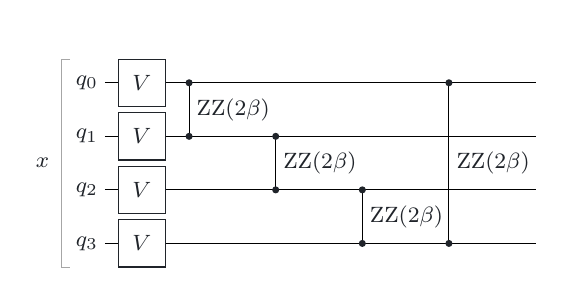
\begin{tikzpicture}[x=1mm,y=-1mm]
\path[use as bounding box] (0,0) rectangle (65,31.5);
% The four displayed qubits form the x register, not the full 2D address.
\draw[group rule] (5.4,4)--(4.3,4)--(4.3,30.4)--(5.4,30.4);
\node[anchor=east,font=\fontsize{8}{9.5}\selectfont] at (2.8,17.2) {$x$};
\foreach \j in {0,1,2,3}{
 \pgfmathsetmacro{\yy}{7+6.8*\j}
 \node[anchor=east,font=\fontsize{8}{9.5}\selectfont] at (9,\yy) {$q_\j$};
 \draw[line width=.4pt] (9.8,\yy)--(64.5,\yy);
 \squaregate{14.5}{\yy}{V}
}
% Standard ZZ(theta) interaction symbols; theta=2 beta, including the ring closure.
\foreach \xx/\ja/\jb in {20.5/0/1,31.5/1/2,42.5/2/3,53.5/3/0}{
 \pgfmathsetmacro{\ya}{7+6.8*\ja}
 \pgfmathsetmacro{\yb}{7+6.8*\jb}
 \pgfmathsetmacro{\ym}{(\ya+\yb)/2}
 \draw[line width=.4pt] (\xx,\ya)--(\xx,\yb);
 \fill[Ink] (\xx,\ya) circle[radius=.45mm] (\xx,\yb) circle[radius=.45mm];
 \node[anchor=west,font=\fontsize{8}{9.5}\selectfont] at (\xx+.9,\ym) {$\mathrm{ZZ}(2\beta)$};
}
\end{tikzpicture}
\end{document}
